\documentclass[11pt]{article}

% ---------------------------------------------------------------------------
% Political Analysis Letter submission.
% Word budget: <=2,500 words total (abstract + body + figure legends +
% footnotes; references and table-cell content excluded). Single-anonymized:
% no author name/affiliation in this file -- see pa_titlepage.tex, submitted
% separately and removed for peer review. <=3 display items (here: 1 figure,
% 1 table). Citation style: Chicago author-date (natbib + chicago.bst).
% ---------------------------------------------------------------------------
\usepackage{fontspec}
\usepackage{microtype}
\usepackage[margin=1in]{geometry}
\usepackage{graphicx}
\usepackage{amsmath}
\usepackage{booktabs}
\usepackage{array}
\usepackage{caption}
\usepackage{float}
\usepackage[colorlinks=true, linkcolor=black, citecolor=black, urlcolor=blue]{hyperref}
\usepackage{xurl}
\usepackage[authoryear,round]{natbib}
\bibpunct{(}{)}{;}{a}{}{,}

\setlength{\parindent}{0pt}
\setlength{\parskip}{0.6em}

\title{\textbf{An error budget for political-bias measurement in large
language models}}
\author{}
\date{}

\begin{document}

\maketitle

\begin{abstract}
Large language models are widely reported to lean left of centre, replicated
across dozens of studies. We show this is substantially a property of
measurement. Administering the Political Compass and 8Values to 19 models,
60 times each (2,280 administrations), we decompose a measured political
position into variance from model identity, instrument choice, and trial
noise. Instrument and axis choice accounts for 52\% of variance (95\% CI
[35\%, 72\%]) and model identity for only 13\% ([0.02\%, 22\%]): which
questionnaire an auditor picks moves a score four times more than which
model is audited. The two instruments also fail convergent validity:
$r=-0.26$ for shared constructs versus $r=+0.52$ for distinct ones on the
same instrument. Crossing two further instruments, SapplyValues and Pew
2026 Political Typology, into the same model collapses the pooled
model-identity share to 1.89\%. Three additional factors, asker identity,
instrument contamination, and response format, each explain more variance
in their factorial designs than model identity explains under the standard
protocol. Reported bias magnitudes are therefore not comparable across
studies using different instruments, and every factor examined explains
more of a score than the model producing it does. We propose a minimum
reporting standard for such audits.
\end{abstract}

Large language models now mediate political information for hundreds of
millions of people, and a substantial literature reports they lean left of
centre, replicated across model families, providers, and languages
\citep{rozado2024, motoki2024, hartmann2023, feng2023, buyl2026,
peng2026beyond, sakhawat2026polalign}. Each assumption behind this
measurement has since been challenged in isolation: models accommodate the
political identity they infer for the asker \citep{tornberg2026sycophancy};
the instruments themselves appear in pretraining data
\citep{bianchi2026plasticity}; forced-choice framing produces answers models
do not give when responding freely \citep{rottger2024}. None has been
quantified against the others, so the field has no estimate of how much of a
reported score is the model and how much is the apparatus. The closest
existing study administers three instruments to 26 models and obtains a
comparable model-versus-prompt split, but measures each cell once, so trial
noise cannot be separated from the instrument term
\citep{sakhawat2026polalign}; repeating each cell and scoring against each
instrument's own authoritative engine, rather than an approximate formula, is
what makes the noise term below possible.

We supply that estimate. Administering the Political Compass and 8Values to
19 models from 11 organizations, spanning open and closed weights and
roughly two orders of magnitude in price, 60 times each (2{,}280
administrations), we decompose a measured political position into variance
from model identity, instrument and axis choice, and residual trial noise,
each with a 95\% CI from a cluster bootstrap over the 19 models. Pooled
across instruments, instrument and axis choice accounts for 52.2\% of
variance ([35.0\%, 71.9\%]) and model identity for only 13.0\% ([0.02\%,
21.9\%]) (Fig.~\ref{fig:error-budget}a; Table~\ref{tab:factors}): which
questionnaire an auditor picks moves a reported score roughly four times
more than which model is audited, and residual trial-to-trial noise (34.8\%,
[18.9\%, 49.3\%]) exceeds the model term. Conditional on a fixed axis, where
the between-instrument term is removed by construction, model identity
accounts for 66.6\% of remaining variance (Fig.~\ref{fig:error-budget}b):
models are clearly separable once the instrument is held constant, and both
figures are correct, but they answer different questions, and only the
first governs comparisons across studies using different instruments.

The two instruments are not interchangeable measures of one underlying
position. A multi-trait multi-method analysis finds convergent
validity---the same construct measured by both instruments---averaging
$r=-0.26$ across the 19 models, against $r=+0.52$ for discriminant validity
(different constructs, same instrument); the Campbell--Fiske ordering, which
requires the first to exceed the second, is inverted. Crossing two further
instruments, SapplyValues and Pew Research Center's 2026 Political
Typology, scored by driving Pew's live public quiz and reading off its own
classification rather than reimplementing its unpublished clustering
procedure, into the same crossed random-effects model collapses the pooled
model-identity share further, to 1.89\% (8{,}640 administrations;
Table~\ref{tab:factors}).\footnote{Automating Pew's live quiz at this scale
(18 models $\times$ 10 trials) is a distinct question from the survey items'
own reuse terms and plausibly exceeds ordinary personal use of that
interactive tool; we disclose this explicitly (web appendix, Ethics
Declarations).} The collapse is driven by SapplyValues actively disagreeing
with Political Compass on model ranking ($\rho=-0.49$), not by Pew's
coarser ordinal scale diluting the signal: adding SapplyValues alone drops
the model share to 0.49\%, adding Pew alone only to 8.21\%.

Three further apparatus components, each demonstrated only in isolation in
the prior literature, are larger than the model term when measured directly
on the same models (Table~\ref{tab:factors}). Framing the asker's identity
---conservative, progressive, apolitical, journalist, academic researcher,
or none---explains more variance ($\eta^2=0.79$, [0.65, 0.93]) than model
identity does under the field's standard unattributed condition
($\eta^2=0.56$--$0.73$); accommodation is asymmetric, moving scores 2.9--6.7
times further from baseline for a conservative framing than a progressive
one. Sense-inverting instrument items with the scoring key flipped produces
a Contamination Index averaging 0.046 ([0.038, 0.055]) of the instrument's
own range, with 17 of 18 models shifting on at least one axis after
correction, and a companion memorisation probe finds a 16.6\% verbatim
item-completion rate. Free-text elicitation, judged onto the same scale,
versus a forced label explains more variance (39\%, [0.02, 0.74]) than
model identity within the same design (23\%, [0.04, 0.52]).

None of these three factors is folded into the pooled budget above, since
each was collected as its own factorial against the field's standard
baseline rather than crossed with instrument simultaneously; doing so is
the natural next step and would likely push the already-small model share
down further still. That is the direction every factor examined has
pushed, and none has pushed the other way.

We are not arguing models are politically neutral, nor that any specific
published estimate is wrong, nor that a questionnaire score predicts
real-world behaviour: a separate, dual-instrument study finds voting-advice
questionnaires and concrete referendum votes disagree
\citep{barmettler2026instrument}, a behavioural-validity question this
design does not test. Within a single study using one instrument, model
identity is clearly measurable and rank orderings are meaningful. The
failure is transportability: published magnitudes are not comparable across
studies using different instruments, askers, or elicitation formats, and
every apparatus component we examined explains more of a reported score
than the model producing it does.

We propose that a political-bias audit report, at minimum: the instrument,
named; the asker condition, including the absence of one; the repetition
count and dispersion, in the instrument's own units; a variance
decomposition across whatever was varied; a contamination check; and
item-level, not only axis-level, results. Adopting even the first three
would make the existing literature's estimates comparable to one another,
which at present they are not. Full methods, the complete four-instrument
crossing, and item-response-theory, prompt-robustness, and
open-ended-generation checks that corroborate these results are in the web
appendix.

\begin{figure}[H]
\centering
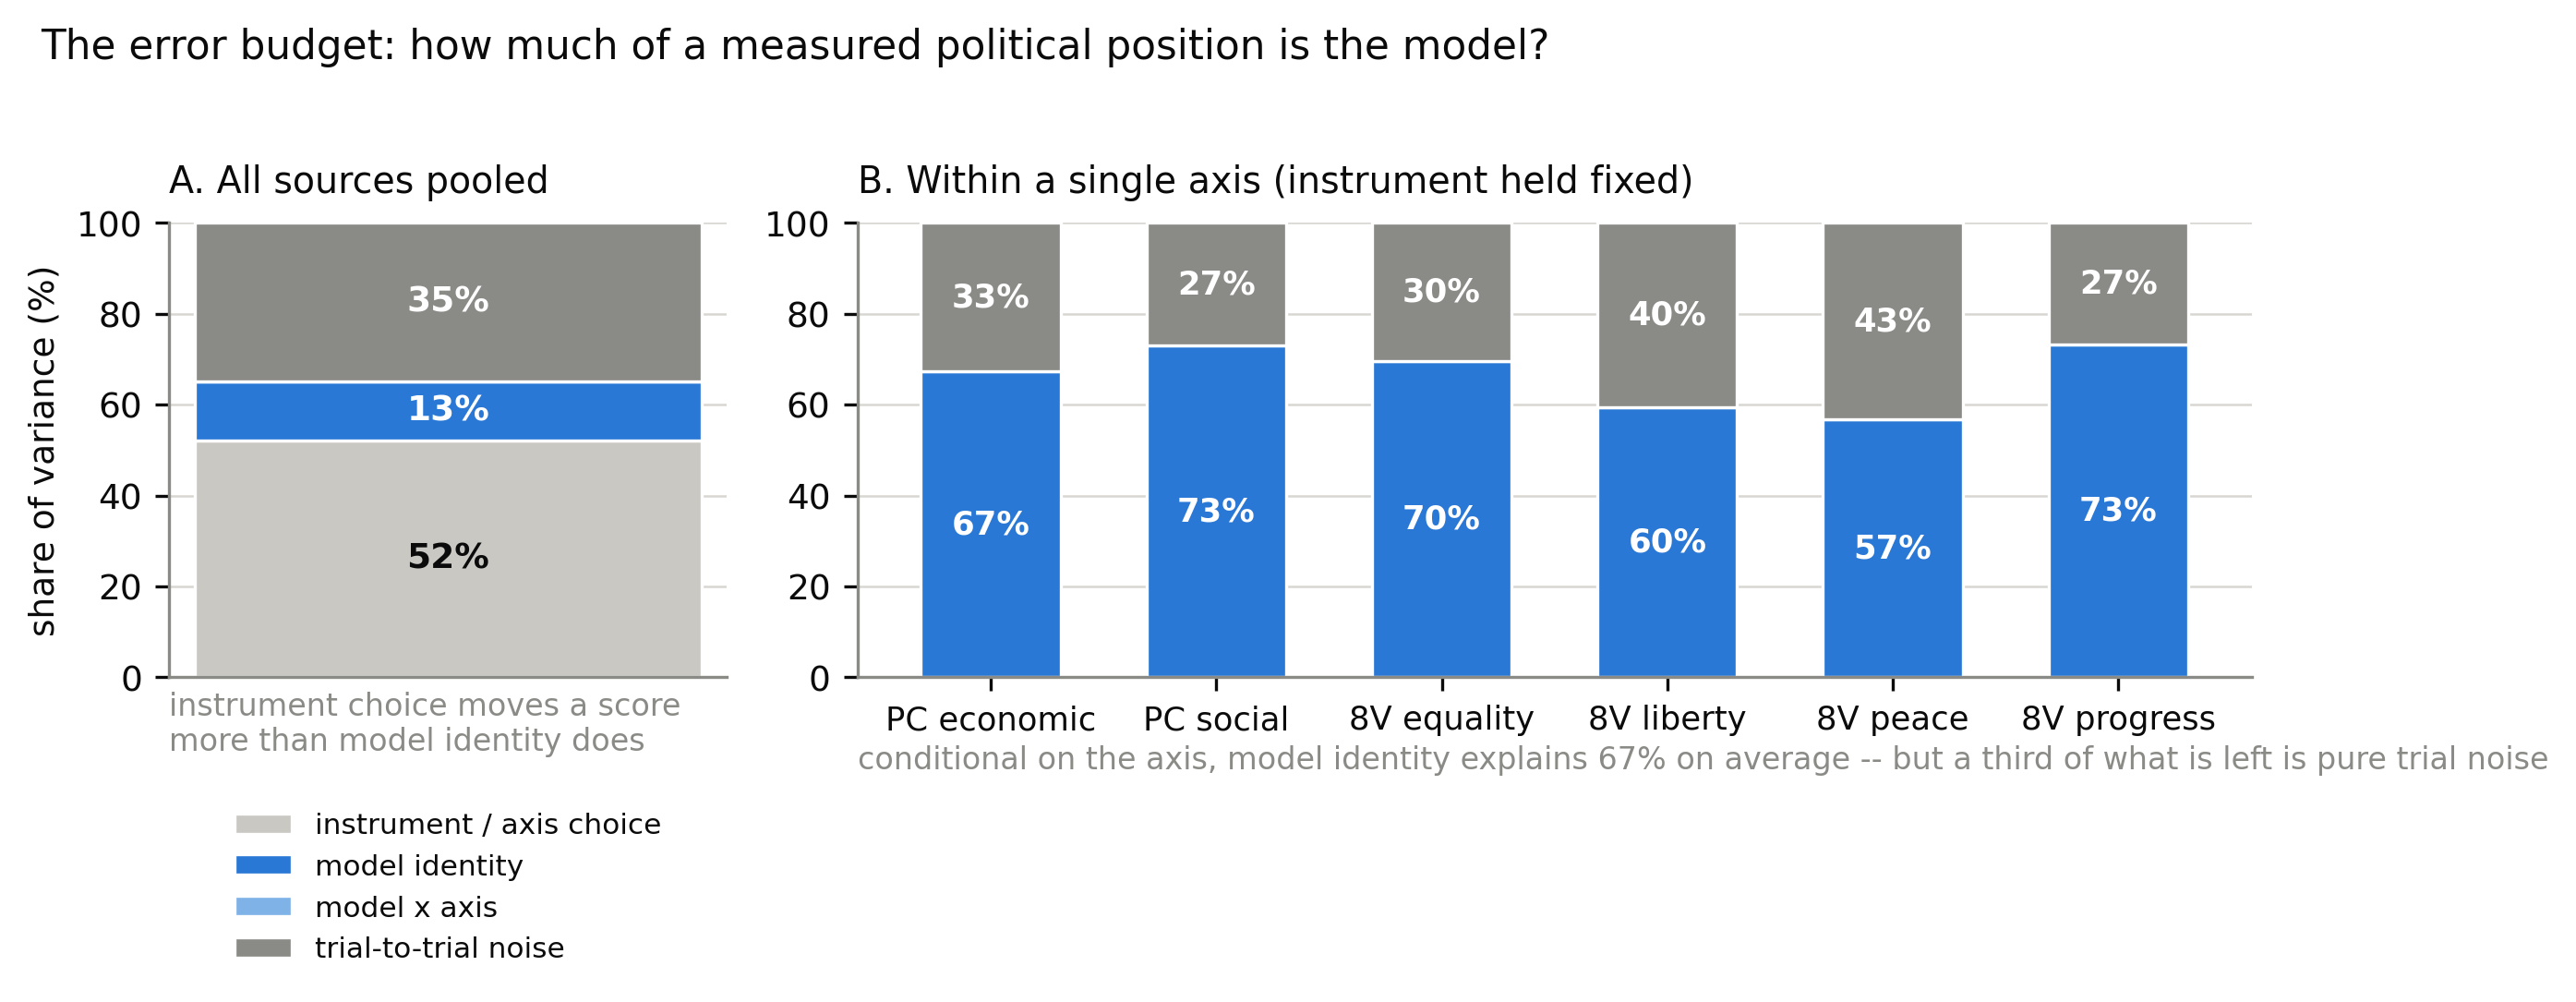
\includegraphics[width=0.85\textwidth]{figures/fig6_error_budget.png}
\caption{\textbf{The error budget.} Variance components of a measured
political position, from a crossed random-effects model on 2{,}280
administrations. (\textbf{a}) Pooled across instruments: instrument and
axis choice accounts for 52\% of variance (95\% CI [35\%, 72\%]), model
identity for 13\% ([0.02\%, 22\%]), residual trial noise for 35\% ([19\%,
49\%]); cluster bootstrap over 19 models, 2{,}000 resamples.
(\textbf{b}) Within a single axis, where the between-instrument term is
removed by construction, model identity accounts for 57--73\%. Panel (a)
governs comparison across studies using different instruments; panel (b)
governs comparison within one study.}
\label{fig:error-budget}
\end{figure}

\begin{table}[H]
\centering
\caption{Every measurement factor examined explains more variance than
model identity does under the field's standard protocol. Model identity's
share is reported under whichever baseline each factor's own design used;
intervals are cluster bootstraps over models. Full designs in the web
appendix.}
\label{tab:factors}
\footnotesize
\begin{tabular}{lp{3.6cm}p{3.6cm}r}
\toprule
Factor & Model identity & Factor itself & $n$ \\
\midrule
Instrument (2 instruments) & 13.0\% [0.02, 21.9] & 52.2\% [35.0, 71.9] & 2{,}280 \\
Instrument (4 instruments) & 1.89\% [0.0, 6.0] & --- & 8{,}640 \\
Asker identity & $\eta^2$ 0.56--0.73 (unattrib.) & $\eta^2$ 0.79 [0.65, 0.93] & 2{,}160 \\
Response format & $\eta^2$ 0.23 [0.04, 0.52] & $\eta^2$ 0.39 [0.02, 0.74] & 4{,}320 \\
Instrument contamination & --- & CI 0.046 [0.038, 0.055]; 17/18 models & 1{,}080 \\
\bottomrule
\end{tabular}
\end{table}

\bibliographystyle{chicago}
\bibliography{references}

\end{document}
